%%%%%%%%%%%%%%%%%%%%%%%%%%%%%% -*- Mode: Latex -*- %%%%%%%%%%%%%%%%%%%%%%%%%%%%
%% 04-14.tex -- Thesis white paper - software inspections
%% Author          : Aaron A. Kagawa
%% Created On      : Mon Sep 23 11:52:28 2004
%% Last Modified By: Aaron Kagawa
%% Last Modified On: Sat Nov 20 13:21:38 2004
%% RCS: $Id$
%%%%%%%%%%%%%%%%%%%%%%%%%%%%%%%%%%%%%%%%%%%%%%%%%%%%%%%%%%%%%%%%%%%%%%%%%%%%%%
%%   Copyright (C) 2004 Aaron A. Kagawa
%%%%%%%%%%%%%%%%%%%%%%%%%%%%%%%%%%%%%%%%%%%%%%%%%%%%%%%%%%%%%%%%%%%%%%%%%%%%%%%
%% 

\documentclass[11pt,twocolumn]{article} 
% Psfig/TeX 
\def\PsfigVersion{1.9}
% dvips version
%
% All psfig/tex software, documentation, and related files
% in this distribution of psfig/tex are 
% Copyright 1987, 1988, 1991 Trevor J. Darrell
%
% Permission is granted for use and non-profit distribution of psfig/tex 
% providing that this notice is clearly maintained. The right to
% distribute any portion of psfig/tex for profit or as part of any commercial
% product is specifically reserved for the author(s) of that portion.
%
% *** Feel free to make local modifications of psfig as you wish,
% *** but DO NOT post any changed or modified versions of ``psfig''
% *** directly to the net. Send them to me and I'll try to incorporate
% *** them into future versions. If you want to take the psfig code 
% *** and make a new program (subject to the copyright above), distribute it, 
% *** (and maintain it) that's fine, just don't call it psfig.
%
% Bugs and improvements to trevor@media.mit.edu.
%
% Thanks to Greg Hager (GDH) and Ned Batchelder for their contributions
% to the original version of this project.
%
% Modified by J. Daniel Smith on 9 October 1990 to accept the
% %%BoundingBox: comment with or without a space after the colon.  Stole
% file reading code from Tom Rokicki's EPSF.TEX file (see below).
%
% More modifications by J. Daniel Smith on 29 March 1991 to allow the
% the included PostScript figure to be rotated.  The amount of
% rotation is specified by the "angle=" parameter of the \psfig command.
%
% Modified by Robert Russell on June 25, 1991 to allow users to specify
% .ps filenames which don't yet exist, provided they explicitly provide
% boundingbox information via the \psfig command. Note: This will only work
% if the "file=" parameter follows all four "bb???=" parameters in the
% command. This is due to the order in which psfig interprets these params.
%
%  3 Jul 1991	JDS	check if file already read in once
%  4 Sep 1991	JDS	fixed incorrect computation of rotated
%			bounding box
% 25 Sep 1991	GVR	expanded synopsis of \psfig
% 14 Oct 1991	JDS	\fbox code from LaTeX so \psdraft works with TeX
%			changed \typeout to \ps@typeout
% 17 Oct 1991	JDS	added \psscalefirst and \psrotatefirst
%

% From: gvr@cs.brown.edu (George V. Reilly)
%
% \psdraft	draws an outline box, but doesn't include the figure
%		in the DVI file.  Useful for previewing.
%
% \psfull	includes the figure in the DVI file (default).
%
% \psscalefirst width= or height= specifies the size of the figure
% 		before rotation.
% \psrotatefirst (default) width= or height= specifies the size of the
% 		 figure after rotation.  Asymetric figures will
% 		 appear to shrink.
%
% \psfigurepath#1	sets the path to search for the figure
%
% \psfig
% usage: \psfig{file=, figure=, height=, width=,
%			bbllx=, bblly=, bburx=, bbury=,
%			rheight=, rwidth=, clip=, angle=, silent=}
%
%	"file" is the filename.  If no path name is specified and the
%		file is not found in the current directory,
%		it will be looked for in directory \psfigurepath.
%	"figure" is a synonym for "file".
%	By default, the width and height of the figure are taken from
%		the BoundingBox of the figure.
%	If "width" is specified, the figure is scaled so that it has
%		the specified width.  Its height changes proportionately.
%	If "height" is specified, the figure is scaled so that it has
%		the specified height.  Its width changes proportionately.
%	If both "width" and "height" are specified, the figure is scaled
%		anamorphically.
%	"bbllx", "bblly", "bburx", and "bbury" control the PostScript
%		BoundingBox.  If these four values are specified
%               *before* the "file" option, the PSFIG will not try to
%               open the PostScript file.
%	"rheight" and "rwidth" are the reserved height and width
%		of the figure, i.e., how big TeX actually thinks
%		the figure is.  They default to "width" and "height".
%	The "clip" option ensures that no portion of the figure will
%		appear outside its BoundingBox.  "clip=" is a switch and
%		takes no value, but the `=' must be present.
%	The "angle" option specifies the angle of rotation (degrees, ccw).
%	The "silent" option makes \psfig work silently.
%

% check to see if macros already loaded in (maybe some other file says
% "\input psfig") ...
\ifx\undefined\psfig\else\endinput\fi

%
% from a suggestion by eijkhout@csrd.uiuc.edu to allow
% loading as a style file. Changed to avoid problems
% with amstex per suggestion by jbence@math.ucla.edu

\let\LaTeXAtSign=\@
\let\@=\relax
\edef\psfigRestoreAt{\catcode`\@=\number\catcode`@\relax}
%\edef\psfigRestoreAt{\catcode`@=\number\catcode`@\relax}
\catcode`\@=11\relax
\newwrite\@unused
\def\ps@typeout#1{{\let\protect\string\immediate\write\@unused{#1}}}
\ps@typeout{psfig/tex \PsfigVersion}

%% Here's how you define your figure path.  Should be set up with null
%% default and a user useable definition.

\def\figurepath{./}
\def\psfigurepath#1{\edef\figurepath{#1}}

%
% @psdo control structure -- similar to Latex @for.
% I redefined these with different names so that psfig can
% be used with TeX as well as LaTeX, and so that it will not 
% be vunerable to future changes in LaTeX's internal
% control structure,
%
\def\@nnil{\@nil}
\def\@empty{}
\def\@psdonoop#1\@@#2#3{}
\def\@psdo#1:=#2\do#3{\edef\@psdotmp{#2}\ifx\@psdotmp\@empty \else
    \expandafter\@psdoloop#2,\@nil,\@nil\@@#1{#3}\fi}
\def\@psdoloop#1,#2,#3\@@#4#5{\def#4{#1}\ifx #4\@nnil \else
       #5\def#4{#2}\ifx #4\@nnil \else#5\@ipsdoloop #3\@@#4{#5}\fi\fi}
\def\@ipsdoloop#1,#2\@@#3#4{\def#3{#1}\ifx #3\@nnil 
       \let\@nextwhile=\@psdonoop \else
      #4\relax\let\@nextwhile=\@ipsdoloop\fi\@nextwhile#2\@@#3{#4}}
\def\@tpsdo#1:=#2\do#3{\xdef\@psdotmp{#2}\ifx\@psdotmp\@empty \else
    \@tpsdoloop#2\@nil\@nil\@@#1{#3}\fi}
\def\@tpsdoloop#1#2\@@#3#4{\def#3{#1}\ifx #3\@nnil 
       \let\@nextwhile=\@psdonoop \else
      #4\relax\let\@nextwhile=\@tpsdoloop\fi\@nextwhile#2\@@#3{#4}}
% 
% \fbox is defined in latex.tex; so if \fbox is undefined, assume that
% we are not in LaTeX.
% Perhaps this could be done better???
\ifx\undefined\fbox
% \fbox code from modified slightly from LaTeX
\newdimen\fboxrule
\newdimen\fboxsep
\newdimen\ps@tempdima
\newbox\ps@tempboxa
\fboxsep = 3pt
\fboxrule = .4pt
\long\def\fbox#1{\leavevmode\setbox\ps@tempboxa\hbox{#1}\ps@tempdima\fboxrule
    \advance\ps@tempdima \fboxsep \advance\ps@tempdima \dp\ps@tempboxa
   \hbox{\lower \ps@tempdima\hbox
  {\vbox{\hrule height \fboxrule
          \hbox{\vrule width \fboxrule \hskip\fboxsep
          \vbox{\vskip\fboxsep \box\ps@tempboxa\vskip\fboxsep}\hskip 
                 \fboxsep\vrule width \fboxrule}
                 \hrule height \fboxrule}}}}
\fi
%
%%%%%%%%%%%%%%%%%%%%%%%%%%%%%%%%%%%%%%%%%%%%%%%%%%%%%%%%%%%%%%%%%%%
% file reading stuff from epsf.tex
%   EPSF.TEX macro file:
%   Written by Tomas Rokicki of Radical Eye Software, 29 Mar 1989.
%   Revised by Don Knuth, 3 Jan 1990.
%   Revised by Tomas Rokicki to accept bounding boxes with no
%      space after the colon, 18 Jul 1990.
%   Portions modified/removed for use in PSFIG package by
%      J. Daniel Smith, 9 October 1990.
%
\newread\ps@stream
\newif\ifnot@eof       % continue looking for the bounding box?
\newif\if@noisy        % report what you're making?
\newif\if@atend        % %%BoundingBox: has (at end) specification
\newif\if@psfile       % does this look like a PostScript file?
%
% PostScript files should start with `%!'
%
{\catcode`\%=12\global\gdef\epsf@start{%!}}
\def\epsf@PS{PS}
%
\def\epsf@getbb#1{%
%
%   The first thing we need to do is to open the
%   PostScript file, if possible.
%
\openin\ps@stream=#1
\ifeof\ps@stream\ps@typeout{Error, File #1 not found}\else
%
%   Okay, we got it. Now we'll scan lines until we find one that doesn't
%   start with %. We're looking for the bounding box comment.
%
   {\not@eoftrue \chardef\other=12
    \def\do##1{\catcode`##1=\other}\dospecials \catcode`\ =10
    \loop
       \if@psfile
	  \read\ps@stream to \epsf@fileline
       \else{
	  \obeyspaces
          \read\ps@stream to \epsf@tmp\global\let\epsf@fileline\epsf@tmp}
       \fi
       \ifeof\ps@stream\not@eoffalse\else
%
%   Check the first line for `%!'.  Issue a warning message if its not
%   there, since the file might not be a PostScript file.
%
       \if@psfile\else
       \expandafter\epsf@test\epsf@fileline:. \\%
       \fi
%
%   We check to see if the first character is a % sign;
%   if so, we look further and stop only if the line begins with
%   `%%BoundingBox:' and the `(atend)' specification was not found.
%   That is, the only way to stop is when the end of file is reached,
%   or a `%%BoundingBox: llx lly urx ury' line is found.
%
          \expandafter\epsf@aux\epsf@fileline:. \\%
       \fi
   \ifnot@eof\repeat
   }\closein\ps@stream\fi}%
%
% This tests if the file we are reading looks like a PostScript file.
%
\long\def\epsf@test#1#2#3:#4\\{\def\epsf@testit{#1#2}
			\ifx\epsf@testit\epsf@start\else
\ps@typeout{Warning! File does not start with `\epsf@start'.  It may not be a PostScript file.}
			\fi
			\@psfiletrue} % don't test after 1st line
%
%   We still need to define the tricky \epsf@aux macro. This requires
%   a couple of magic constants for comparison purposes.
%
{\catcode`\%=12\global\let\epsf@percent=%\global\def\epsf@bblit{%BoundingBox}}
%
%
%   So we're ready to check for `%BoundingBox:' and to grab the
%   values if they are found.  We continue searching if `(at end)'
%   was found after the `%BoundingBox:'.
%
\long\def\epsf@aux#1#2:#3\\{\ifx#1\epsf@percent
   \def\epsf@testit{#2}\ifx\epsf@testit\epsf@bblit
	\@atendfalse
        \epsf@atend #3 . \\%
	\if@atend	
	   \if@verbose{
		\ps@typeout{psfig: found `(atend)'; continuing search}
	   }\fi
        \else
        \epsf@grab #3 . . . \\%
        \not@eoffalse
        \global\no@bbfalse
        \fi
   \fi\fi}%
%
%   Here we grab the values and stuff them in the appropriate definitions.
%
\def\epsf@grab #1 #2 #3 #4 #5\\{%
   \global\def\epsf@llx{#1}\ifx\epsf@llx\empty
      \epsf@grab #2 #3 #4 #5 .\\\else
   \global\def\epsf@lly{#2}%
   \global\def\epsf@urx{#3}\global\def\epsf@ury{#4}\fi}%
%
% Determine if the stuff following the %%BoundingBox is `(atend)'
% J. Daniel Smith.  Copied from \epsf@grab above.
%
\def\epsf@atendlit{(atend)} 
\def\epsf@atend #1 #2 #3\\{%
   \def\epsf@tmp{#1}\ifx\epsf@tmp\empty
      \epsf@atend #2 #3 .\\\else
   \ifx\epsf@tmp\epsf@atendlit\@atendtrue\fi\fi}


% End of file reading stuff from epsf.tex
%%%%%%%%%%%%%%%%%%%%%%%%%%%%%%%%%%%%%%%%%%%%%%%%%%%%%%%%%%%%%%%%%%%

%%%%%%%%%%%%%%%%%%%%%%%%%%%%%%%%%%%%%%%%%%%%%%%%%%%%%%%%%%%%%%%%%%%
% trigonometry stuff from "trig.tex"
\chardef\psletter = 11 % won't conflict with \begin{letter} now...
\chardef\other = 12

\newif \ifdebug %%% turn me on to see TeX hard at work ...
\newif\ifc@mpute %%% don't need to compute some values
\c@mputetrue % but assume that we do

\let\then = \relax
\def\r@dian{pt }
\let\r@dians = \r@dian
\let\dimensionless@nit = \r@dian
\let\dimensionless@nits = \dimensionless@nit
\def\internal@nit{sp }
\let\internal@nits = \internal@nit
\newif\ifstillc@nverging
\def \Mess@ge #1{\ifdebug \then \message {#1} \fi}

{ %%% Things that need abnormal catcodes %%%
	\catcode `\@ = \psletter
	\gdef \nodimen {\expandafter \n@dimen \the \dimen}
	\gdef \term #1 #2 #3%
	       {\edef \t@ {\the #1}%%% freeze parameter 1 (count, by value)
		\edef \t@@ {\expandafter \n@dimen \the #2\r@dian}%
				   %%% freeze parameter 2 (dimen, by value)
		\t@rm {\t@} {\t@@} {#3}%
	       }
	\gdef \t@rm #1 #2 #3%
	       {{%
		\count 0 = 0
		\dimen 0 = 1 \dimensionless@nit
		\dimen 2 = #2\relax
		\Mess@ge {Calculating term #1 of \nodimen 2}%
		\loop
		\ifnum	\count 0 < #1
		\then	\advance \count 0 by 1
			\Mess@ge {Iteration \the \count 0 \space}%
			\Multiply \dimen 0 by {\dimen 2}%
			\Mess@ge {After multiplication, term = \nodimen 0}%
			\Divide \dimen 0 by {\count 0}%
			\Mess@ge {After division, term = \nodimen 0}%
		\repeat
		\Mess@ge {Final value for term #1 of 
				\nodimen 2 \space is \nodimen 0}%
		\xdef \Term {#3 = \nodimen 0 \r@dians}%
		\aftergroup \Term
	       }}
	\catcode `\p = \other
	\catcode `\t = \other
	\gdef \n@dimen #1pt{#1} %%% throw away the ``pt''
}

\def \Divide #1by #2{\divide #1 by #2} %%% just a synonym

\def \Multiply #1by #2%%% allows division of a dimen by a dimen
       {{%%% should really freeze parameter 2 (dimen, passed by value)
	\count 0 = #1\relax
	\count 2 = #2\relax
	\count 4 = 65536
	\Mess@ge {Before scaling, count 0 = \the \count 0 \space and
			count 2 = \the \count 2}%
	\ifnum	\count 0 > 32767 %%% do our best to avoid overflow
	\then	\divide \count 0 by 4
		\divide \count 4 by 4
	\else	\ifnum	\count 0 < -32767
		\then	\divide \count 0 by 4
			\divide \count 4 by 4
		\else
		\fi
	\fi
	\ifnum	\count 2 > 32767 %%% while retaining reasonable accuracy
	\then	\divide \count 2 by 4
		\divide \count 4 by 4
	\else	\ifnum	\count 2 < -32767
		\then	\divide \count 2 by 4
			\divide \count 4 by 4
		\else
		\fi
	\fi
	\multiply \count 0 by \count 2
	\divide \count 0 by \count 4
	\xdef \product {#1 = \the \count 0 \internal@nits}%
	\aftergroup \product
       }}

\def\r@duce{\ifdim\dimen0 > 90\r@dian \then   % sin(x+90) = sin(180-x)
		\multiply\dimen0 by -1
		\advance\dimen0 by 180\r@dian
		\r@duce
	    \else \ifdim\dimen0 < -90\r@dian \then  % sin(-x) = sin(360+x)
		\advance\dimen0 by 360\r@dian
		\r@duce
		\fi
	    \fi}

\def\Sine#1%
       {{%
	\dimen 0 = #1 \r@dian
	\r@duce
	\ifdim\dimen0 = -90\r@dian \then
	   \dimen4 = -1\r@dian
	   \c@mputefalse
	\fi
	\ifdim\dimen0 = 90\r@dian \then
	   \dimen4 = 1\r@dian
	   \c@mputefalse
	\fi
	\ifdim\dimen0 = 0\r@dian \then
	   \dimen4 = 0\r@dian
	   \c@mputefalse
	\fi
%
	\ifc@mpute \then
        	% convert degrees to radians
		\divide\dimen0 by 180
		\dimen0=3.141592654\dimen0
%
		\dimen 2 = 3.1415926535897963\r@dian %%% a well-known constant
		\divide\dimen 2 by 2 %%% we only deal with -pi/2 : pi/2
		\Mess@ge {Sin: calculating Sin of \nodimen 0}%
		\count 0 = 1 %%% see power-series expansion for sine
		\dimen 2 = 1 \r@dian %%% ditto
		\dimen 4 = 0 \r@dian %%% ditto
		\loop
			\ifnum	\dimen 2 = 0 %%% then we've done
			\then	\stillc@nvergingfalse 
			\else	\stillc@nvergingtrue
			\fi
			\ifstillc@nverging %%% then calculate next term
			\then	\term {\count 0} {\dimen 0} {\dimen 2}%
				\advance \count 0 by 2
				\count 2 = \count 0
				\divide \count 2 by 2
				\ifodd	\count 2 %%% signs alternate
				\then	\advance \dimen 4 by \dimen 2
				\else	\advance \dimen 4 by -\dimen 2
				\fi
		\repeat
	\fi		
			\xdef \sine {\nodimen 4}%
       }}

% Now the Cosine can be calculated easily by calling \Sine
\def\Cosine#1{\ifx\sine\UnDefined\edef\Savesine{\relax}\else
		             \edef\Savesine{\sine}\fi
	{\dimen0=#1\r@dian\advance\dimen0 by 90\r@dian
	 \Sine{\nodimen 0}
	 \xdef\cosine{\sine}
	 \xdef\sine{\Savesine}}}	      
% end of trig stuff
%%%%%%%%%%%%%%%%%%%%%%%%%%%%%%%%%%%%%%%%%%%%%%%%%%%%%%%%%%%%%%%%%%%%

\def\psdraft{
	\def\@psdraft{0}
	%\ps@typeout{draft level now is \@psdraft \space . }
}
\def\psfull{
	\def\@psdraft{100}
	%\ps@typeout{draft level now is \@psdraft \space . }
}

\psfull

\newif\if@scalefirst
\def\psscalefirst{\@scalefirsttrue}
\def\psrotatefirst{\@scalefirstfalse}
\psrotatefirst

\newif\if@draftbox
\def\psnodraftbox{
	\@draftboxfalse
}
\def\psdraftbox{
	\@draftboxtrue
}
\@draftboxtrue

\newif\if@prologfile
\newif\if@postlogfile
\def\pssilent{
	\@noisyfalse
}
\def\psnoisy{
	\@noisytrue
}
\psnoisy
%%% These are for the option list.
%%% A specification of the form a = b maps to calling \@p@@sa{b}
\newif\if@bbllx
\newif\if@bblly
\newif\if@bburx
\newif\if@bbury
\newif\if@height
\newif\if@width
\newif\if@rheight
\newif\if@rwidth
\newif\if@angle
\newif\if@clip
\newif\if@verbose
\def\@p@@sclip#1{\@cliptrue}


\newif\if@decmpr

%%% GDH 7/26/87 -- changed so that it first looks in the local directory,
%%% then in a specified global directory for the ps file.
%%% RPR 6/25/91 -- changed so that it defaults to user-supplied name if
%%% boundingbox info is specified, assuming graphic will be created by
%%% print time.
%%% TJD 10/19/91 -- added bbfile vs. file distinction, and @decmpr flag

\def\@p@@sfigure#1{\def\@p@sfile{null}\def\@p@sbbfile{null}
	        \openin1=#1.bb
		\ifeof1\closein1
	        	\openin1=\figurepath#1.bb
			\ifeof1\closein1
			        \openin1=#1
				\ifeof1\closein1%
				       \openin1=\figurepath#1
					\ifeof1
					   \ps@typeout{Error, File #1 not found}
						\if@bbllx\if@bblly
				   		\if@bburx\if@bbury
			      				\def\@p@sfile{#1}%
			      				\def\@p@sbbfile{#1}%
							\@decmprfalse
				  	   	\fi\fi\fi\fi
					\else\closein1
				    		\def\@p@sfile{\figurepath#1}%
				    		\def\@p@sbbfile{\figurepath#1}%
						\@decmprfalse
	                       		\fi%
			 	\else\closein1%
					\def\@p@sfile{#1}
					\def\@p@sbbfile{#1}
					\@decmprfalse
			 	\fi
			\else
				\def\@p@sfile{\figurepath#1}
				\def\@p@sbbfile{\figurepath#1.bb}
				\@decmprtrue
			\fi
		\else
			\def\@p@sfile{#1}
			\def\@p@sbbfile{#1.bb}
			\@decmprtrue
		\fi}

\def\@p@@sfile#1{\@p@@sfigure{#1}}

\def\@p@@sbbllx#1{
		%\ps@typeout{bbllx is #1}
		\@bbllxtrue
		\dimen100=#1
		\edef\@p@sbbllx{\number\dimen100}
}
\def\@p@@sbblly#1{
		%\ps@typeout{bblly is #1}
		\@bbllytrue
		\dimen100=#1
		\edef\@p@sbblly{\number\dimen100}
}
\def\@p@@sbburx#1{
		%\ps@typeout{bburx is #1}
		\@bburxtrue
		\dimen100=#1
		\edef\@p@sbburx{\number\dimen100}
}
\def\@p@@sbbury#1{
		%\ps@typeout{bbury is #1}
		\@bburytrue
		\dimen100=#1
		\edef\@p@sbbury{\number\dimen100}
}
\def\@p@@sheight#1{
		\@heighttrue
		\dimen100=#1
   		\edef\@p@sheight{\number\dimen100}
		%\ps@typeout{Height is \@p@sheight}
}
\def\@p@@swidth#1{
		%\ps@typeout{Width is #1}
		\@widthtrue
		\dimen100=#1
		\edef\@p@swidth{\number\dimen100}
}
\def\@p@@srheight#1{
		%\ps@typeout{Reserved height is #1}
		\@rheighttrue
		\dimen100=#1
		\edef\@p@srheight{\number\dimen100}
}
\def\@p@@srwidth#1{
		%\ps@typeout{Reserved width is #1}
		\@rwidthtrue
		\dimen100=#1
		\edef\@p@srwidth{\number\dimen100}
}
\def\@p@@sangle#1{
		%\ps@typeout{Rotation is #1}
		\@angletrue
%		\dimen100=#1
		\edef\@p@sangle{#1} %\number\dimen100}
}
\def\@p@@ssilent#1{ 
		\@verbosefalse
}
\def\@p@@sprolog#1{\@prologfiletrue\def\@prologfileval{#1}}
\def\@p@@spostlog#1{\@postlogfiletrue\def\@postlogfileval{#1}}
\def\@cs@name#1{\csname #1\endcsname}
\def\@setparms#1=#2,{\@cs@name{@p@@s#1}{#2}}
%
% initialize the defaults (size the size of the figure)
%
\def\ps@init@parms{
		\@bbllxfalse \@bbllyfalse
		\@bburxfalse \@bburyfalse
		\@heightfalse \@widthfalse
		\@rheightfalse \@rwidthfalse
		\def\@p@sbbllx{}\def\@p@sbblly{}
		\def\@p@sbburx{}\def\@p@sbbury{}
		\def\@p@sheight{}\def\@p@swidth{}
		\def\@p@srheight{}\def\@p@srwidth{}
		\def\@p@sangle{0}
		\def\@p@sfile{} \def\@p@sbbfile{}
		\def\@p@scost{10}
		\def\@sc{}
		\@prologfilefalse
		\@postlogfilefalse
		\@clipfalse
		\if@noisy
			\@verbosetrue
		\else
			\@verbosefalse
		\fi
}
%
% Go through the options setting things up.
%
\def\parse@ps@parms#1{
	 	\@psdo\@psfiga:=#1\do
		   {\expandafter\@setparms\@psfiga,}}
%
% Compute bb height and width
%
\newif\ifno@bb
\def\bb@missing{
	\if@verbose{
		\ps@typeout{psfig: searching \@p@sbbfile \space  for bounding box}
	}\fi
	\no@bbtrue
	\epsf@getbb{\@p@sbbfile}
        \ifno@bb \else \bb@cull\epsf@llx\epsf@lly\epsf@urx\epsf@ury\fi
}	
\def\bb@cull#1#2#3#4{
	\dimen100=#1 bp\edef\@p@sbbllx{\number\dimen100}
	\dimen100=#2 bp\edef\@p@sbblly{\number\dimen100}
	\dimen100=#3 bp\edef\@p@sbburx{\number\dimen100}
	\dimen100=#4 bp\edef\@p@sbbury{\number\dimen100}
	\no@bbfalse
}
% rotate point (#1,#2) about (0,0).
% The sine and cosine of the angle are already stored in \sine and
% \cosine.  The result is placed in (\p@intvaluex, \p@intvaluey).
\newdimen\p@intvaluex
\newdimen\p@intvaluey
\def\rotate@#1#2{{\dimen0=#1 sp\dimen1=#2 sp
%            	calculate x' = x \cos\theta - y \sin\theta
		  \global\p@intvaluex=\cosine\dimen0
		  \dimen3=\sine\dimen1
		  \global\advance\p@intvaluex by -\dimen3
% 		calculate y' = x \sin\theta + y \cos\theta
		  \global\p@intvaluey=\sine\dimen0
		  \dimen3=\cosine\dimen1
		  \global\advance\p@intvaluey by \dimen3
		  }}
\def\compute@bb{
		\no@bbfalse
		\if@bbllx \else \no@bbtrue \fi
		\if@bblly \else \no@bbtrue \fi
		\if@bburx \else \no@bbtrue \fi
		\if@bbury \else \no@bbtrue \fi
		\ifno@bb \bb@missing \fi
		\ifno@bb \ps@typeout{FATAL ERROR: no bb supplied or found}
			\no-bb-error
		\fi
		%
%\ps@typeout{BB: \@p@sbbllx, \@p@sbblly, \@p@sbburx, \@p@sbbury} 
%
% store height/width of original (unrotated) bounding box
		\count203=\@p@sbburx
		\count204=\@p@sbbury
		\advance\count203 by -\@p@sbbllx
		\advance\count204 by -\@p@sbblly
		\edef\ps@bbw{\number\count203}
		\edef\ps@bbh{\number\count204}
		%\ps@typeout{ psbbh = \ps@bbh, psbbw = \ps@bbw }
		\if@angle 
			\Sine{\@p@sangle}\Cosine{\@p@sangle}
	        	{\dimen100=\maxdimen\xdef\r@p@sbbllx{\number\dimen100}
					    \xdef\r@p@sbblly{\number\dimen100}
			                    \xdef\r@p@sbburx{-\number\dimen100}
					    \xdef\r@p@sbbury{-\number\dimen100}}
%
% Need to rotate all four points and take the X-Y extremes of the new
% points as the new bounding box.
                        \def\minmaxtest{
			   \ifnum\number\p@intvaluex<\r@p@sbbllx
			      \xdef\r@p@sbbllx{\number\p@intvaluex}\fi
			   \ifnum\number\p@intvaluex>\r@p@sbburx
			      \xdef\r@p@sbburx{\number\p@intvaluex}\fi
			   \ifnum\number\p@intvaluey<\r@p@sbblly
			      \xdef\r@p@sbblly{\number\p@intvaluey}\fi
			   \ifnum\number\p@intvaluey>\r@p@sbbury
			      \xdef\r@p@sbbury{\number\p@intvaluey}\fi
			   }
%			lower left
			\rotate@{\@p@sbbllx}{\@p@sbblly}
			\minmaxtest
%			upper left
			\rotate@{\@p@sbbllx}{\@p@sbbury}
			\minmaxtest
%			lower right
			\rotate@{\@p@sbburx}{\@p@sbblly}
			\minmaxtest
%			upper right
			\rotate@{\@p@sbburx}{\@p@sbbury}
			\minmaxtest
			\edef\@p@sbbllx{\r@p@sbbllx}\edef\@p@sbblly{\r@p@sbblly}
			\edef\@p@sbburx{\r@p@sbburx}\edef\@p@sbbury{\r@p@sbbury}
%\ps@typeout{rotated BB: \r@p@sbbllx, \r@p@sbblly, \r@p@sbburx, \r@p@sbbury}
		\fi
		\count203=\@p@sbburx
		\count204=\@p@sbbury
		\advance\count203 by -\@p@sbbllx
		\advance\count204 by -\@p@sbblly
		\edef\@bbw{\number\count203}
		\edef\@bbh{\number\count204}
		%\ps@typeout{ bbh = \@bbh, bbw = \@bbw }
}
%
% \in@hundreds performs #1 * (#2 / #3) correct to the hundreds,
%	then leaves the result in @result
%
\def\in@hundreds#1#2#3{\count240=#2 \count241=#3
		     \count100=\count240	% 100 is first digit #2/#3
		     \divide\count100 by \count241
		     \count101=\count100
		     \multiply\count101 by \count241
		     \advance\count240 by -\count101
		     \multiply\count240 by 10
		     \count101=\count240	%101 is second digit of #2/#3
		     \divide\count101 by \count241
		     \count102=\count101
		     \multiply\count102 by \count241
		     \advance\count240 by -\count102
		     \multiply\count240 by 10
		     \count102=\count240	% 102 is the third digit
		     \divide\count102 by \count241
		     \count200=#1\count205=0
		     \count201=\count200
			\multiply\count201 by \count100
		 	\advance\count205 by \count201
		     \count201=\count200
			\divide\count201 by 10
			\multiply\count201 by \count101
			\advance\count205 by \count201
			%
		     \count201=\count200
			\divide\count201 by 100
			\multiply\count201 by \count102
			\advance\count205 by \count201
			%
		     \edef\@result{\number\count205}
}
\def\compute@wfromh{
		% computing : width = height * (bbw / bbh)
		\in@hundreds{\@p@sheight}{\@bbw}{\@bbh}
		%\ps@typeout{ \@p@sheight * \@bbw / \@bbh, = \@result }
		\edef\@p@swidth{\@result}
		%\ps@typeout{w from h: width is \@p@swidth}
}
\def\compute@hfromw{
		% computing : height = width * (bbh / bbw)
	        \in@hundreds{\@p@swidth}{\@bbh}{\@bbw}
		%\ps@typeout{ \@p@swidth * \@bbh / \@bbw = \@result }
		\edef\@p@sheight{\@result}
		%\ps@typeout{h from w : height is \@p@sheight}
}
\def\compute@handw{
		\if@height 
			\if@width
			\else
				\compute@wfromh
			\fi
		\else 
			\if@width
				\compute@hfromw
			\else
				\edef\@p@sheight{\@bbh}
				\edef\@p@swidth{\@bbw}
			\fi
		\fi
}
\def\compute@resv{
		\if@rheight \else \edef\@p@srheight{\@p@sheight} \fi
		\if@rwidth \else \edef\@p@srwidth{\@p@swidth} \fi
		%\ps@typeout{rheight = \@p@srheight, rwidth = \@p@srwidth}
}
%		
% Compute any missing values
\def\compute@sizes{
	\compute@bb
	\if@scalefirst\if@angle
% at this point the bounding box has been adjsuted correctly for
% rotation.  PSFIG does all of its scaling using \@bbh and \@bbw.  If
% a width= or height= was specified along with \psscalefirst, then the
% width=/height= value needs to be adjusted to match the new (rotated)
% bounding box size (specifed in \@bbw and \@bbh).
%    \ps@bbw       width=
%    -------  =  ---------- 
%    \@bbw       new width=
% so `new width=' = (width= * \@bbw) / \ps@bbw; where \ps@bbw is the
% width of the original (unrotated) bounding box.
	\if@width
	   \in@hundreds{\@p@swidth}{\@bbw}{\ps@bbw}
	   \edef\@p@swidth{\@result}
	\fi
	\if@height
	   \in@hundreds{\@p@sheight}{\@bbh}{\ps@bbh}
	   \edef\@p@sheight{\@result}
	\fi
	\fi\fi
	\compute@handw
	\compute@resv}

%
% \psfig
% usage : \psfig{file=, height=, width=, bbllx=, bblly=, bburx=, bbury=,
%			rheight=, rwidth=, clip=}
%
% "clip=" is a switch and takes no value, but the `=' must be present.
\def\psfig#1{\vbox {
	% do a zero width hard space so that a single
	% \psfig in a centering enviornment will behave nicely
	%{\setbox0=\hbox{\ }\ \hskip-\wd0}
	%
	\ps@init@parms
	\parse@ps@parms{#1}
	\compute@sizes
	%
	\ifnum\@p@scost<\@psdraft{
		%
		\special{ps::[begin] 	\@p@swidth \space \@p@sheight \space
				\@p@sbbllx \space \@p@sbblly \space
				\@p@sbburx \space \@p@sbbury \space
				startTexFig \space }
		\if@angle
			\special {ps:: \@p@sangle \space rotate \space} 
		\fi
		\if@clip{
			\if@verbose{
				\ps@typeout{(clip)}
			}\fi
			\special{ps:: doclip \space }
		}\fi
		\if@prologfile
		    \special{ps: plotfile \@prologfileval \space } \fi
		\if@decmpr{
			\if@verbose{
				\ps@typeout{psfig: including \@p@sfile.Z \space }
			}\fi
			\special{ps: plotfile "`zcat \@p@sfile.Z" \space }
		}\else{
			\if@verbose{
				\ps@typeout{psfig: including \@p@sfile \space }
			}\fi
			\special{ps: plotfile \@p@sfile \space }
		}\fi
		\if@postlogfile
		    \special{ps: plotfile \@postlogfileval \space } \fi
		\special{ps::[end] endTexFig \space }
		% Create the vbox to reserve the space for the figure.
		\vbox to \@p@srheight sp{
		% 1/92 TJD Changed from "true sp" to "sp" for magnification.
			\hbox to \@p@srwidth sp{
				\hss
			}
		\vss
		}
	}\else{
		% draft figure, just reserve the space and print the
		% path name.
		\if@draftbox{		
			% Verbose draft: print file name in box
			\hbox{\frame{\vbox to \@p@srheight sp{
			\vss
			\hbox to \@p@srwidth sp{ \hss \@p@sfile \hss }
			\vss
			}}}
		}\else{
			% Non-verbose draft
			\vbox to \@p@srheight sp{
			\vss
			\hbox to \@p@srwidth sp{\hss}
			\vss
			}
		}\fi	



	}\fi
}}
\psfigRestoreAt
\let\@=\LaTeXAtSign




\usepackage{/export/home/csdl/tex/icse2003/latex8}
\usepackage{times}
%% A verbatim-like environment which allows font changes
%%\usepackage{alltt}
%% New LaTeX2e graphics support
\usepackage[final]{graphicx}
% uncomment the % away on next line to produce the final camera-ready version
% and uncomment the \thispagestyle{empty} following \maketitle
\pagestyle{empty}

\begin{document}

\title{Limited Resource Software Inspections}

\author{\protect\begin{tabular}{ccc}
Aaron A. Kagawa \\
\end{tabular}\\
\em  Collaborative Software Development Laboratory \\
\em  Department of Information and Computer Sciences \\
\em  University of Hawai'i \\
\em  Honolulu, HI 96822 \\
\em  kagawaa@hawaii.edu}
\maketitle
\thispagestyle{empty}

\begin{abstract}  % 200 words
Imagine that your project manager has budgeted 200 person-hours for the
next month to inspect newly created source code.  Unfortunately, in order
to inspect all of the documents adequately, you estimate that it will
take 400 person-hours.  However, your manager refuses to increase the
budgeted resources for the inspections.  How do you decide
which documents to inspect and which documents to skip?

The classic definition of Inspection, does not provide any advice on how to
handle this situation. For example, the notion of entry criteria used in
Software Inspection determines when documents are ready for inspection
rather than if inspection is needed at all \cite{Ebenau94}.

%% I could talk about previous approaches here. Sampling and Up-Stream documents

This proposed research will investigate how to prioritize inspection
resources and apply them to areas of the system that need them the most.
It is commonly assumed that defects are not uniformly distributed across
all documents in a system - that a relatively small subset of a system
accounts for a relatively large proportion of defects \cite{Boehm01}.  If
inspection resources are limited, then it will be most effective to
identify and inspect the defect-prone areas.

To accomplish this research, I will construct an evaluation framework based
upon automated process and product measures to distinguish documents that
are in ``most need of inspection'' from those in ``least need of
inspection''.  Some examples of the process and product measures that are
being considered include: reported defects, unit tests, test coverage,
active time, and number of changes. Based on this framework I hypothesize,
that code deemed in most need of inspection will generate more critical
issues than code deemed least need of inspection.

%% Each measure acts as an indedendent variable for determining the inspection
%% candidacy of a document and can be assigned an individual weight. 

Each measure affects the determination of ``most and least'' differently.
For example, suppose that test coverage should be weighted more than active
time. Therefore, weights of each measure will be calibrated based on my
initial guesses.  My research will employ a very simple evaluation
strategy, which includes selecting code to inspect, analyzing the results,
and adjusting the calibration of the measures.

There are three milestones that measure my progress in this reasearch.
Milestone 1: implementation of Hackystat Extension, January 2005.
Milestone 2: completed evaluation, March 2005. Milestone 3: thesis
submission and defense, April 2005.
\end{abstract}

%%%%%%%%%%%%%%%%%%%%%%%%%%%%% -*- Mode: Latex -*- %%%%%%%%%%%%%%%%%%%%%%%%%%%%
%% 04-14-intro.tex -- Priority Ranked Software Inspection
%% Author          : Aaron A. Kagawa
%% Created On      : Mon Sep 23 11:52:28 2004
%% Last Modified By: Aaron Kagawa
%% Last Modified On: Sat Feb  5 13:25:36 2005
%% RCS: $Id$
%%%%%%%%%%%%%%%%%%%%%%%%%%%%%%%%%%%%%%%%%%%%%%%%%%%%%%%%%%%%%%%%%%%%%%%%%%%%%%
%%   Copyright (C) 2004 Aaron A. Kagawa
%%%%%%%%%%%%%%%%%%%%%%%%%%%%%%%%%%%%%%%%%%%%%%%%%%%%%%%%%%%%%%%%%%%%%%%%%%%%%%%


\chapter{Introduction}
Software inspection is defined as: ``A formal evaluation technique in which
software requirements, design, or code are examined in detail by a person
or group other than the author to detect faults, violations of development
standards, and other problems...'' \cite{Gilb93}. Software inspection, or
software review as it is sometimes called, can have fantastic results:
``Rigorous inspection can remove up to 90 percent of errors from a software
product before the fist test case is run'' \cite{Glass03, Bush90}.

Since Michael Fagan invented the inspection technique in 1976, there have
been many variations on the general concept of inspection. We now have
Fagan Inspection \cite{Fagan76}, Software Inspection \cite{Gilb93},
High-Impact Inspection, Phased Inspection, ``regular'' software inspection,
software reviews, code walkthroughs, inspections without meetings, and many
more different twists on the original concept.  Each of these techniques
claim to be the best inspection method for their certain circumstances. For
example, some argue that the inspection meeting is a waste of time and
resources \cite{Johnson97, Johnson98, Votta93}. Others argue that the
inspection meeting is critical for supporting social and educational
aspects of inspection \cite{Johnson98}.

My research is different from traditional inspection research. Instead of
asking how to conduct the inspection process, I ask how to determine what
to inspect, when to conduct inspections, and more importantly if inspection
is really needed for a particular piece of code. In this proposal, I will
describe how the selection of a document for inspection can create problems
for organizations with limited inspection resources. I will then propose a
new inspection document selection technique called Priority Ranked
Inspection and evaluate its effectiveness.


%%Since the introduction of inspections by Michael Fagan, there have been
%%numerous views, descriptions, and process that have been proposed by
%%various authors and researchers. Some of these include; Fagan Inspections
%%\cite{Fagan76}, Software Inspections \cite{Gilb93}, High-Impact
%%Inspections, and Phased Inspections just to name a few. Throughout this
%%paper I will use the lower cased inspection to represent all inspection
%%techniques.

\section{The Problem of Limited Resources for Software Inspections}
The use of software inspection has reported outstanding results in
improving productivity and quality. One study has found that when the
inspection process is followed correctly, up to 95 percent of defects can
be removed before entering the testing phase \cite{Bush90}. In another
success story, the Jet Propulsion Laboratory (JPL) adopted inspection to
identify defects and experienced a savings of 7.5 million dollars by
conducting 300 inspections \cite{Bush90a}. This statistic is very
impressive. However, what is not emphasized is each inspection had an
average total cost of 28 hours. Using that average cost, the total cost for
JPL's inspection process was 8,400 hours or roughly 4 years of work.

The JPL experience illustrates a fundamental problem with inspections:
better results come from substantial investment \cite{Gilb93}. Not all
organizations have the time or the money to invest in full or complete
inspections. In most cases, organizations have limited funds or resources
that can be devoted to inspections. For example, a manager may only have
200 hours of a project schedule to allocate towards quality assurance
including inspections. Such organizations must decide how to best utilize
their limited inspection resources. This realistic management of
inspections directly contradicts the classical inspection adage of ``when a
document is ready, you should inspect it''. The bottom line is that most
organizations cannot inspect every document.

The traditional inspection process begins with the initiation phase, or
sometimes called the planning stage, in which authors volunteer their
documents for inspection \cite {Gilb93}. A inspection leader checks the
document against entry criteria to determine if the document is ready for
inspection \cite{Ebenau94, Gilb93}. Again this process works very well for
organizations, like JPL, that have the resources to inspect every document
after every significant change. However, I believe that this phase of
inspection is a major problem for organizations that do not have the
necessary resources, because the process does not consider that some
documents are ``better'' to inspect than others. A simple illustration of
this fact is that 80 percent of defects come from 20 percent of the system
\cite{Boehm01}.  Thus, volunteering a document from the defect-prone 20
percent will likely be ``more in need of inspection'' than any other part
of the system.

Furthermore, the current literature \cite{Ebenau94, Wiegers02, Gilb93} on
inspections does not provide specific insights into the trade-offs between
inspecting some documents and not inspecting others.  However, Tom Gilb and
Dorothy Graham provide two recommendations to use when inspection resources
are limited; sampling and emphasizing up-stream documents \cite{Gilb93}.
The use of sampling involves inspecting various areas of a system to
identify areas of interest. Up-stream documents are documents that define
high-level requirements or designs.  Inspecting up-stream documents ensures
that the requirements are correct before any implementation is started.
Although, these are very useful recommendations, they do not provide much
specific guidance of how best to use limited inspection resources.

%%For example, consider the following scenario:
%%\begin{quotation}
%%  \textit{The FooBar organization has enough resources available to conduct
%%    two inspections a week. However, this organization creates and finishes
%%    10 different documents each week. How do they select 2 documents from
%%    the possible 10 to inspect? To be fair to all developers they use a
%%    round-robin type approach by allowing a different developer to
%%    volunteer a document for inspection. This approach is fairly successful
%%    and at least they are conducting inspections. But, are they inspecting
%%    the right documents? Obviously, this organization is unavoidably
%%    letting 8 documents slip through the inspection-crack and could be
%%    releasing documents that have critical defects.}
%%\end{quotation}


\section{The Priority Ranked Inspection Approach}
To address some of the problems associated with conducting inspections with
limited resources, I propose a new inspection process called ``Priority
Ranked Inspection'', (PRI). The primary goal of PRI is to optimize the
selection of documents for inspection by distingushing what documents are
``more in need of inspection'' (MINI) versus documents that are ``less in
need of inspection'' (LINI). In addition, PRI will rank each document
according to this determination in hopes of prioritizing the documents that
need to be inspected. The converse is also true: PRI will identify
documents that might not need to be inspected.

As I have shown in the previous section, it is extremely difficult for
organizations with limited inspection resources to inspect every document
before it exits the development process. Therefore, unlike traditional
inspection process, PRI does not require that all documents be inspected.
Instead, PRI is intended to help these organizations in two ways. First,
PRI is intended to be able to identify documents in the current development
process that need to be inspected. This will allow organizations to make an
educated guess at what documents need to be inspected and what documents
can be skipped. Second, it is unavoidable that some documents with critical
defects will finish the development process without being inspected.
Therefore, PRI is also intended to identify documents for inspection
regardless if a document is currently in the development process or not.

%%In the same ways that Software Inspection \cite{Gilb93} is an inspection
%%process, Priority Ranked Inspection is also an inspection
%%process. However, the differences between the two inspection processes lie
%%in the recognition that not all organizations have the necessary resources 
%%to inspect everything. Therefore, PRI is tailored to the organizations with 
%%limited resources. 

There are four primary steps in the Priority Ranked Inspection (PRI)
process. The following list is short description of each of the steps. The
following sub-sections provide a summary description of each step.

\begin{enumerate}
\item The creation of the PRI weighting function, which distinguishes
  MINI documents from LINI documents. The weighting function design
  includes two steps: 
\begin{enumerate}
\item Selection of product and process measures to use in the PRI
  weighting function.
\item Creation of a numerical weighting system that assigns a weight for
  each measure and the calibration of this weighting system.
\end{enumerate}
\item The selection of a document for inspection based on the PRI
  ranking.
\item The actual inspection of the selected document.
\item Adjustment of product and process measure selection and
  calibration based on the results of the inspection.
\end{enumerate}


\subsection{Step 1a: Selection of Product and Process Measures}
The PRI weighting function which distinguishes MINI documents from LINI
documents will be generated automatically from various product and process
measures. Product measures are usually obtainable from direct analysis of
source code.  For example, lines of code, complexity, and number of
children are a few examples of product measures. On the other hand, process
measures are collected from the actual software development process. The
amount of developer 'effort' and the number of defects are examples of
process measures. One might ask, what specific measures should PRI
consider? The answer: it depends on the specific situation. Different
projects and organizations could have a different set of measures in
defining the optimum PRI weighting function and ranking. Therefore, a major
component of the PRI process is the selection of the measures.

Software quality measures are one example of the type of product and
process measures that could be used in PRI. Software inspection has two
primary goals; increase quality and productivity. For this research I am
primarily concerned with increasing quality. The successful inspection of a
document has two main results: finding defects which, once removed,
increases software quality or not finding defects thus indicating high
software quality. Software quality is vaguely defined as ``the degree to
which software possesses a desired combination of attributes''
\cite{IEEEGlossary83}. Some of the possible measures of quality include:
portability, reliability, efficiency, usability, testability,
understandability, and modifiability \cite{Glass03}. Some other widely
accepted measures of quality include defect density and complexity.
Whatever definition used for quality, inspections aim to increase or
validate the level of quality in software.  Therefore, the same measures of
software quality will also provide good indications of what documents need
inspection. For example, finding documents that have low portability,
reliability, efficiency, usability, testability, understandability, and
modifiability would provide a good indication that the documents are MINI.

Based on the previous example, the quality-specific product and process
measures can be extracted and used in the PRI weighting function. Table
\ref{table:step1a} is an example of the PRI ranking of a software project
that contains three documents.  Presented in the table are the measures and
values that are used in the PRI ranking. Due to constraints of the paper
size, the table presents only a couple of the measures discussed above.
However, any number of measures can be used in the PRI weighting function.

\begin{table}[htbp]
  \caption{Step 1a - Example PRI ranking - After Measure Selection}
  \label{table:step1a}
  \begin{center}
    \begin{tabular}{|l|l|l|l|l|l|l|} \hline
      {\bf Document} & {\bf PRI Ranking} & {\bf Reliability} & 
      {\bf Efficiency} & {\bf Testability} & {\bf ...} \\ \hline
Foo.java & MINI & 3 & 4 & 2 & ...  \\ \hline
Bar.java & LINI & 4 & 2 & 6 & ...  \\ \hline
Baz.java & LINI & 1 & 2 & 3 & ...  \\ \hline
    \end{tabular}
  \end{center}
\end{table}

Table \ref{table:step1a} is an illustration of a fictitious PRI ranking.
See Chapter \ref{chapter:system}: Hackystat PRI Extension for more details
about the exact calculations necessary to create a PRI weighting function
and ranking.


\subsection{Step 1b: Calibration of the Product and Process Measures}
Only selecting what measures to be used in the PRI weighting function is
not adequate, because some measures are more important than others. For
example, an organization may find that testability has a greater positive
impact on the PRI weighting function than efficiency. Therefore, Step 1b of
the PRI process is the calibration of the measures' importance. The
calibration of the measures is based on a numerical weighting system. Each
measure will be assigned a numerical weight and will be individually
calibrated. The numerical weighting system and the calibration creates a
PRI ranking, which provides a priority ranking of the documents.

Using the same example (Table \ref{table:step1a}) from the previous
section, imagine that the organization has found testability to be a
leading indicator in defect prevention. Therefore, the calibration is
adjusted and the values of testability are given a higher weight than the
other measures. This finding changes the PRI weighting function and
ranking. The following table (Table \ref{table:step1b}) shows the new PRI
ranking after the calibration.

\label{table:step1b_trial}
\begin{table}[htbp]
  \caption{Step 1b - Example PRI ranking - After Measure Calibration}
  \label{table:step1b}
  \begin{center}
    \begin{tabular}{|l|l|l|l|l|l|l|} \hline
      {\bf Document} & {\bf PRI Ranking} & {\bf Reliability} & 
      {\bf Efficiency} & {\bf Testability} & {\bf ...} \\ \hline
Bar.java & MINI & 4 & 2 & 6 & ...  \\ \hline
Foo.java & MINI & 3 & 4 & 2 & ...  \\ \hline
Baz.java & LINI & 1 & 2 & 3 & ...  \\ \hline
    \end{tabular}
  \end{center}
\end{table}

Notice that, as a result of the calibration, the PRI ranking for Bar.java
has changed from LINI to MINI. This illustrates that the PRI weighting
function and ranking can be flexible and that it has the pontential to
reflect different development processes within different organizations.


\subsection{Step 2: Selecting a Document for Inspection Based on the PRI
  Ranking} After the PRI weighting function and ranking is in place,
an organization may use PRI to select documents for inspection. To select a
document for inspection they simply consult the PRI ranking and find a MINI
document (a document deemed more in need of inspection). This ranking will
help constrain the number of possible documents that can be considered for
inspection.

For example, in the example presented in Table \ref{table:step1b}, an
organization should select Bar.java for the inspection, because it ranked
the highest of the three documents. During the next inspection meeting,
Foo.java should be inspected. However, Baz.java could be skipped, thus
saving inspection resources.

Using the PRI ranking to select documents for inspection has three primary
benefits. First, it can enhance the selection or the volunteering process
of a document for inspection. Second, it can identify documents for
inspection that a volunteering process typically does not. Third,
inspecting a MINI document will generate more critical defects than
inspecting a LINI document.


\subsection{Step 3: Conducting an Inspection of the Selected Document}
Once the document is selected, a traditional inspection process can begin.
PRI does not have any special processes for this step. An organization can
choose to use any traditional inspection process (i.e., Software
Inspection, Fagan Inspection, In-Process Inspection). In other words, the
PRI process is an outer layer that wraps around an already established
inspection process to enhance the selection of documents.  Therefore, in
this research I will not discuss or evaluate traditional inspection
concepts like; inspection leaders, preparation time, etc.


\subsection{Step 4: Adjustment of the Measure Selection and Calibration}
After the inspection of a document, the results can be used to further
improve the PRI weighting function and ranking. For example, if the PRI
weighting function appears to be incorrect, because it ranked a document as
MINI but no major defects were found, then the PRI weighting function
should be adjusted to classify this document as LINI. This adjustment can
be achieved in two ways. First, one could add more product and process
measures to make the PRI weighting function more robust. Alternatively, one
could calibrate the current measures to refine and correct the PRI
weighting function and ranking.  In either case, an incorrect PRI weighting
function will provide data to help make future PRI weighting functions
better. This process should be an ongoing evolving activity.

For example, consider the example presented with Foo.java, Bar.java, and
Baz.java. If an organization has found results that suggest that efficiency
is a leading indicator of defects, then it should be calibrated with a
higher weight.



\section{The Hackystat PRI Extension}
To successfully use PRI, the determination of MINI and LINI must be
obtainable for a very low cost. In other words, if the weighting function
takes three months to generate, a software project will have long past the
need for those specific recommendations. Therefore, this determination must
be obtained in real-time.

One way of obtaining weighting function values in real-time is through the
use of the Hackystat system. Hackystat is a framework for collecting and
analyzing software product and development process metrics in real-time.
For more information about the Hackystat system see Chapter
\ref{chapter:hackystat}.  For this proposed research, I have created an
extension to the Hackystat system called the Hackystat PRI Extension
(hackyPRI for short). hackyPRI provides a real-time PRI weighting function
and ranking. Figure \ref{fig:intro-WorkspacePRIAnalysis} demonstrates the
PRI weighting function and its ranking for a software project that is
obtainable from the Hackystat PRI Extension.

\begin{figure*}[ht]
  \centering
  \includegraphics[width=1.00\textwidth]{WorkspaceQuality.eps}
  \caption{The Workspace PRI analysis. Workspaces are listed with its
  respective PRI ranking and measures.}
  \label{fig:intro-WorkspacePRIAnalysis}
\end{figure*}

The Hackystat PRI Extension will be implemented to fully support all 4
steps of the PRI process. The next subsections demonstrate how hackyPRI
supports each of the 4 steps. It is important to note that PRI is a
proposed \textit{process}, therefore many different tools can support it.
Using the Hackystat PRI Extension is not required to conduct PRI
inspections.



\subsection{Step 1a: Selection of Product and Process Measures}
The Hackystat system provides a standard set of product and process
measures, these measures are called Sensor Data Types within the Hacksytat
system, and the means of its collection. Initially, I have developed
hackyPRI to use all of the measures obtainable from Hackystat. In addition,
I have begun to implement a several new Hackystat Sensor Data Types
(measures), that I feel will aid the PRI weighting function.

Each column in Figure \ref{fig:intro-WorkspacePRIAnalysis} is a measure
that is obtainable from Hackystat. Each measure will be automatically and
unobtrusively collected by Hackystat and directly fed in to the hackyPRI
extension.


\subsection{Step 1b: Calibration of Product and Process Measures}
Each measure and its numerical weight will be stored within the hackyPRI
extension. The numerical weights are not shown in Figure
\ref{fig:intro-WorkspacePRIAnalysis}. However, the calibration and
weighting system works behind the scenes to rank each document. For
example, the coverage measure is assigned a numerical weight of 3 if the
coverage value equals 100 percent, 2 if the coverage value is below 90
percent, 1 if the coverage value is below 80 percent, and 0 if the coverage
value is below 70 percent. See Chapter \ref{chapter:system} for a detailed
description about the numerical weighting system.


\subsection{Step 2: Selecting a Document for Inspection Based on the PRI
  Ranking} Using the PRI Hackystat analysis, an organization should
select a document at the bottom of the PRI ranking table for inspection.
The higher the document is in the table, the more it is likely to be LINI.


\subsection{Step 3: Conducting an Inspection of the Selected Document}
Once a document is selected it can be inspected. One interesting side
effect of the PRI ranking is that specific statistics and measures
can be presented during the inspection process. For example, if a document
is selected because it has low coverage, then the inspection can focus on
why the coverage is low.

\subsection{Step 4: Adjustment of the Measure Selection and Calibration}
If a document is shown to be incorrectly ranked, then an adjustment of the
PRI weighting function is necessary. This can be accomplished by adding
more Hackystat measures to the PRI weighting function or recalibrating the
numerical weights associated with the measures. See Chapter
\ref{chapter:system} for a detailed description of the calibration process
for the hackyPRI extension.



\section{Thesis Statement}
The thesis statement of this research is as follows; Priority Ranked
Inspection can distinguish documents that are more in need of inspection
(MINI) from others that need inspection less (LINI). This thesis statement
can be decomposed into the following three main claims, which are based on
the intended benefits of PRI.

\begin{enumerate}
\item PRI can enhance the volunteer-based document selection process.
\item PRI can identify documents that need to be inspected that are not
  typically identified by volunteering.
\item Documents that are deemed more in need of inspection (MINI) will
  generate more critical defects than documents deemed less in need of
  inspection (LINI).
\end{enumerate}

My first claim states that PRI can enhance the selection process. In the
traditional inspection process, this selection process is based on a
developer selecting and volunteering a document for inspection.  This claim
is an intended benefit of PRI because in the traditional inspection process
the number of documents that a developer must select from can vary widely.
If PRI can provide the MINI documents, then the developer can focus his
selection on a smaller set of documents.

My second claim states that PRI can identify documents that have slipped
through the cracks in the development process. For an organization with
limited inspection resources it is not possible to inspect every document.
Therefore, it is inevitable that some documents that need to be inspected
have not been.

My third and last claim states that the inspection of MINI documents will
generate more critical defects than LINI documents. This claim is very
important to the PRI process because if this claim is proven to be false,
then the PRI process cannot solve the limited inspection resource problem.



\section{Evaluation}
This section provides a short description of the methodologies used to
evaluate my thesis claims. Chapter \ref{chapter:evaluation}, Evaluation
Methodology provides a detailed explanation of the methodologies and
procedures that will be used in the evaluation of PRI.

I will evaluate the main thesis of this proposed research by testing each
of my three claims. In this evaluation, I will be studying the inspection
process of the Hackystat system developed by the Collaborative Software
Development Laboratory. I will also be using the developers of Hackystat as
subjects in my evaluation.

My first claim states that PRI enhances the volunteer-based document
selection process. To evaluate this claim, I will conduct a qualitative and
quantitative evaluation.  First, I will assess the developers' current
selection process by asking them to rank a few documents based on what
documents they think are more in need of inspection. Then I will provide
them with the PRI ranking of those same documents and ask them which
rankings would they change. After this qualitative evaluation, I will ask
CSDL to inspect a few documents to evaluate the validity of the developers'
subjective ranking and the PRI ranking.

My second claim states that PRI can identify MINI documents that are not
typically identified by the volunteering process. To evaluate this claim, I
will ask CSDL to inspect a few documents that have not been identified in
the previous evaluation.

My third and last claim states that the inspection of MINI documents will
generate more critical defects than LINI documents. Throughout the
previous two studies I will have collected information about approximately
20 inspections. By quantitatively analyzing the results of these
inspections I will be able to provide supporting evidence for this claim.


\section{Structure of the Proposal}
The remainder of this proposed research is as follows. Chapter
\ref{chapter:relatedwork} discusses previous studies that influenced this
research. Chapter \ref{chapter:hackystat} and Chapter \ref{chapter:system}
contains a detailed description of the Hackystat system and the Priority
Ranked Inspection (PRI) Hackystat extension. Chapter
\ref{chapter:evaluation} discusses the evaluation methodology that will be
implemented to evaluate the claims and benefits of PRI. Chapter
\ref{chapter:contribution} discusses the contributions and future
directions of this research. Finally, Chapter \ref{chapter:timeline}
provides a detailed timeline of this proposed research.














% LocalWords:  Kagawa Sep


%%%%%%%%%%%%%%%%%%%%%%%%%%%%%% -*- Mode: Latex -*- %%%%%%%%%%%%%%%%%%%%%%%%%%%%
%% 04-14.tex -- Thesis white paper - software inspections
%% Author          : Aaron A. Kagawa
%% Created On      : Mon Sep 23 11:52:28 2004
%% Last Modified By: Aaron Kagawa
%% Last Modified On: Tue Nov  9 18:43:00 2004
%% RCS: $Id$
%%%%%%%%%%%%%%%%%%%%%%%%%%%%%%%%%%%%%%%%%%%%%%%%%%%%%%%%%%%%%%%%%%%%%%%%%%%%%%
%%   Copyright (C) 2004 Aaron A. Kagawa
%%%%%%%%%%%%%%%%%%%%%%%%%%%%%%%%%%%%%%%%%%%%%%%%%%%%%%%%%%%%%%%%%%%%%%%%%%%%%%%
%% 

\Section{Related Work}


%%%%%%%%%%%%%%%%%%%%%%%%%%%%%% -*- Mode: Latex -*- %%%%%%%%%%%%%%%%%%%%%%%%%%%%
%% 04-14-system.tex -- Thesis white paper - software inspections
%% Author          : Aaron A. Kagawa
%% Created On      : Mon Sep 23 11:52:28 2004
%% Last Modified By: Aaron Kagawa
%% Last Modified On: Sat Nov 20 13:30:04 2004
%% RCS: $Id$
%%%%%%%%%%%%%%%%%%%%%%%%%%%%%%%%%%%%%%%%%%%%%%%%%%%%%%%%%%%%%%%%%%%%%%%%%%%%%%
%%   Copyright (C) 2004 Aaron A. Kagawa
%%%%%%%%%%%%%%%%%%%%%%%%%%%%%%%%%%%%%%%%%%%%%%%%%%%%%%%%%%%%%%%%%%%%%%%%%%%%%%%
%% 

\Section{Hackystat LRSI Extension}
This section provides a short description of the Hackystat LRSI
Extension system. This system extends the functionality of the Hackystat
System to provide the ``most'' and ``least'' need of inspection determinations.

The Hackystat System provides several Sensor Data Types that represent
quantitative data about both the product and development process of a
software project. Using this data I will build attributes that represent
quality. For example, some of the attributes that are currently possible
are the following:

\begin{enumerate}
\item Active Time
\item Number of Changes (Commits)
\item Date of Last Change
\item Number of Inspections
\item Date of Last Inspection
\item Number of Defects
\item Date of Last Defect
\item Lines of Code, Number of Methods, and Number of Classes
\item Lines of Test Code, Number of Test Methods, and Number of Test
Classes
\item Coverage
\item Number of Executed Unit Tests
\item Dependency Metrics
\end{enumerate}

Currently, each of these attributes is collected for each package or
workspace within a specified project. Figure 1 shows several example high
quality (or ``least need of inspection'') workspaces with their respective
attributes of quality.

\begin{figure*}[ht]
  \centering
  \includegraphics[width=1.00\textwidth]{WorkspaceQuality.eps}
  \caption{The Workspace LRSI analysis. Workspaces are listed with its
  respective LRSI level and the attributes that make up its LRSI
  level.
}
  \label{fig:WorkspaceQualityAnalysis}
\end{figure*}

To make the important determination of ``most'' and ``least'' need of
inspection, I assign certain quality levels or numerical weights to the
attributes. For example, if the coverage of a package is below 80 percent,
I assign a ``low'' quality level for that attribute. Likewise, if the
coverage of a package is a 100 percent, then I assign a ``high'' quality
level. ``Low'' is operationalized by a 1, ``high'' is operationalized by a
3, and ``middle ground'' is operationalized by a 2. The system assigns each
attribute a quality level and then assigns each package an aggregated
quality level, which is the sum of the quality levels associated with its
attributes. The packages are then sorted by the packages' aggregate quality
level, sorting the ``most need of inspection'' to the bottom and ``least need
of inspection'' to the top.

There are several issues with the assignment of numerical weights (or
quality levels as I call them) that I still need to address. For example, I
explicitly determine the quality levels using my own subjective measure of
what is low versus high quality. I will need to explore if my subjective
measure is sufficient, if some attributes should be weighted more than
others, or if any other entirely different weighting methods provide more
accurate results.




%%%%%%%%%%%%%%%%%%%%%%%%%%%%%%% -*- Mode: Latex -*- %%%%%%%%%%%%%%%%%%%%%%%%%%%%
%% 04-14-evaluation.tex -- Thesis proposal - PRI 
%% Author          : Aaron A. Kagawa
%% Created On      : Mon Sep 23 11:52:28 2004
%% Last Modified By: Aaron Kagawa
%% Last Modified On: Tue Mar  1 16:53:54 2005
%% RCS: $Id$
%%%%%%%%%%%%%%%%%%%%%%%%%%%%%%%%%%%%%%%%%%%%%%%%%%%%%%%%%%%%%%%%%%%%%%%%%%%%%%
%%   Copyright (C) 2004 Aaron A. Kagawa
%%%%%%%%%%%%%%%%%%%%%%%%%%%%%%%%%%%%%%%%%%%%%%%%%%%%%%%%%%%%%%%%%%%%%%%%%%%%%%%


\chapter{Evaluation Methodology}
\label{chapter:evaluation}
This chapter discusses the proposed evaluation methodology of this
research. The main thesis of this proposed research is that Priority Ranked
Inspection (PRI) can distinguish documents that are more in need of
inspection (MINI) from those less in need of inspection (LINI).

One approach of implementing PRI is through Hackystat, thus I will create a
Hackystat Extension called hackyPRI. This extension will provide a
Hackystat analysis, which will distinguish what documents are MINI from
documents that are LINI.  This determination is based on a ranking function
of different process and product measures. Some measures include: reported
defects, unit tests, test coverage, active time, and number of changes.
Each measure will implement a different ranking function and will be
individually calibrated. See Chapter 4: The Hackystat PRI Extension for
more details.

It is important to note two limitations of this research. First, I am not
defining a set of measures that represent the PRI ranking function for
all software projects. Instead, by using hackyPRI I will be able to go
through a methodology to best calibrate the measures to accurately reflect
the determination for the project I am studying. Second, PRI is more
beneficial for organizations that have limited inspection resources. PRI is
of less use for organizations that have the necessary resources to
thoroughly inspect every document, although this is yet to be studied.


\section{Subjects Used in the Evaluation}
In this evaluation, I will study the implementation and inspection process
of the Hackystat System developed in the Collaborative Software Development
Laboratory (CSDL), of the University of Hawaii at Manoa. Like most
organizations, CSDL's inspection resources are limited and therefore
inspections are conducted, if at all, on a weekly basis regardless of the
number of ``ready'' documents. 

%%In addition, unlike most organizations who
%%conduct Software Inspection and have limited resources, CSDL does not
%%conduct sampling or inspections on up-stream documents to enhance the
%%inspection process as recommended by Tom Gilb \cite{Gilb93}. CSDL does not
%%follow these recommendations for two reasons. First, CSDL does not have
%%enough resources to conduct sampling. Second, Hackystat does not contain
%%many up-stream requirement and design documents.

CSDL primarily inspects source code grouped by Java packages; therefore, I
will use the term 'packages' when referring to CSDL's use of PRI. I will
use the term 'documents' when referring to the general idea of inspections.

Although I am a member of CSDL and have been contributing to Hackystat, I
will minimize any possible data contamination by doing two things. First, I
will ensure that the inspection participants are ``Blind'' to the document
selection method. There are two methods of selection that will be used in
this evaluation; selection without aid of PRI and selection with the aid of
PRI. To accomplish this I will work with inidividual authors to select
documents based on their subjective selection or with the aid of PRI and
keep that decission a secret from the rest of the participants. Second, I
obviously will not participate in the inspections themselves.

%%Second, I will ensure that the request for inspection will not indicate
%%whether the package for inspection was chosen by a developer or with the
%%aid of PRI.  This practice is called ``Double Blind''. The importance of
%%``Double Blind'' is to ensure that the Inspection participants are not
%%influenced conciously or subconciously. The only CSDL member, besides
%%myself, who will know of the method in which a document was chosen is the
%%author.

The use of CSDL in my study indicates another limitation on this research.
The most accurate and thorough evaluation of PRI should inspect
\textit{all} documents to evaluate if PRI correctly classifies MINI and
LINI documents. However, because I am using CSDL's inspection resources,
which are limited, this is not possible.



\section{Evaluation of Thesis Claims}
To evaluate this thesis, I have decomposed it into three claims based upon
the three intended benefits of PRI.

\begin{enumerate}
\item PRI can enhance the volunteer-based document selection process. 
\item PRI can identify documents that need to be inspected that are not
  typically identified by volunteering.
\item MINI documents will generate more critical defects than LINI
  documents.
\end{enumerate}

The following sections will detail the methodologies used to evaluate each
of the three claims.


\subsection{Claim 1: PRI Enhances the Volunteering Process}
\label{sec:claim1}
In the traditional inspection process, developers volunteer their documents
for inspection. In most cases, developers select documents to volunteer to
remove any critical defects before it is released. However, the current
literature does not provide much guidance on which documents should be
volunteered. One of the intended benefits of PRI is the enhancement of the
volunteering process by providing suggestions on what should be inspected.
PRI can do this in two ways. First, it can minimize the number of documents
that should be considered for inspection. Second, it provides a priority
ranking of what documents would be most beneficial to inspect.

PRI can minimize the number of documents that should be considered for
inspection. In Software Inspection \cite{Gilb93}, the number of possible
inspection includes \textit{all} the documents currently moving through the
development cycle.  (This technique tends to emphasize only current
documents and not the highest priority documents for inspection. Claim 2
addresses this issue.)  In PRI, the number of possible documents is
minimized to MINI documents. This reduces the number of possibile
inspections and can be advantageous for organizations that cannot inspect
every document, because it will eliminate the need and more importantly it
limits the possibility of inspecting LINI documents.

As an example of how PRI benefits an organization with limited resources
consider the following fictitious scenario:

\begin{quotation}
  \textit{ The FooBar organization has enough resources available to
    conduct inspections at least once a week. Because this organization
    produces more code than is possible to inspect, they use a round-robin
    approach by allowing a different developer to volunteer a piece of code
    to inspect. This developer must pick a small portion of the code he/she
    is currently working on and this decision is primarily based solely on
    his/her subjective opinions of the code.  }
\end{quotation}

This method works well if the developer can be trusted to pick the right
code to inspect. However, developers often do not know where every critical
defect will appear. In other words, leaving this decision up to the
subjective understanding of a developer maybe error prone. PRI provides an
alternative solution to this limited resource problem.  Instead of leaving
the decision of what code to inspect entirely up to the developer, PRI can
minimize the number of possibilities by providing a smaller area of
selection. For this fictional organization, the developer can find the MINI
documents and choose code from this smaller list.

PRI provides a priority ranking of what documents would be most beneficial
to inspect. This advantage supports the volunteering process by allowing
the developer to prioritize his/her selection of documents. The previous
discussion showed how PRI can minimize the number of documents; and now
that the number is reduced the developer still must select from this
smaller number. To support this selection, PRI ranks the documents
according to the calibration and numerical ranking. For example consider
this scenario:

\begin{quotation}
  \textit{ Developer John Doe is currently working on 10 different
    documents and he wants to volunteer one of them for inspection. He has
    a rough idea of what documents he thinks would be most beneficial for
    inspection but he isn't sure. He consults the PRI ranking and finds
    that 6 of his documents appear to be LINI. In addition, he is able to
    use the rankings to select a MINI document that he believes would
    generate more critical defects.}
\end{quotation}

This scenario illustrates how PRI can enhance the volunteering process by
first minimizing the number of documents that should be considered for
inspection and then prioritizing them.

\subsubsection{Evaluation Methodology} 
To evaluate this claim, I will ask the developers of Hackystat to provide a
numerical ranking, based on their subjective feelings, of what packages
they would volunteer for inspection. With these results I will be able to
compare the developers' subjective rankings against the PRI ranking In
addition, I will present each developer with the results of the hackyPRI
analysis, which provides the PRI weighting fuction and ranking. Then I will
ask the developers to re-rank the packages based on the new information.
This evaluation will indicate whether PRI is really needed. The findings
could indicate that developers can correctly distinguish, using their own
subjective reasoning, what packages need to be inspected.

To conduct this evaluation, I will provide each developer with a list of
Hackystat packages that they are currently working on. This will be
determined by assessing the developers' active time and commits to a
particular package. Given this listing I will ask each developer to provide
a numerical ranking of each package.

The following steps will occur in this evaluation:
\begin{enumerate}
\item Obtain the rankings of packages from each individual developer. I
  will use the questionnaire presented in Appendix
  \ref{appendix:questionnaire} to obtain these rankings.
\item Analyze the difference between the developers' ranking against the
  PRI MINI and LINI determination.
\item Conduct the following inspections: 
\begin{enumerate}
\item Inspect 2 packages, where the developer and the PRI determinations
  agree, that are MINI.
\item Inspect 2 packages, where the developer and the PRI determinations
  agree, that are LINI.
\item Inspect 2 packages where the developer and the PRI determinations
  disagree. The developer provides a low ranking but the PRI claims that
  the package is MINI.
\item Inspect 2 packages where the developer and the PRI determinations
  disagree. The developer provides a high ranking but the PRI claims that
  the package is LINI.
\end{enumerate}
\item Analyze the results of each inspection, which includes correlating
  the number of critical issues generated with both the developer ranking
  and the PRI determination. In addition, I may ask the developers for
  explanations of their rankings where applicable.
\item After each inspection I will adjust PRI calibration or add new
  product and process measures as necessary.
\end{enumerate}

There are three possible results from this evaluation. First, I may find
that developers automatically have a sense of what code is MINI and what
code is LINI. This would indicate that PRI provides little added value.
Second, developers have no idea what code needs to be inspected. The third
possible result represents a middle ground between the two previous
results, sometimes the developers are correct and sometimes they are wrong.
The last two results will indicate that PRI provides some benefit.


In addition, this evaluation will provide more data to refine the
calibration of the PRI weighting function.  For example, if a developer
rates a package very high, but PRI finds the package to be LINI and many
critical issues are found, then this indicates that the PRI weighting
function is flawed. Therefore, the PRI weighting function needs to be
recalibrated to include this document. In addition to calibration, more
process and product measures could be introduced. This event, although
detrimental to the previous PRI weighting function, will provide more data
for calibration and the addition of new measures will hopefully lead to a
better and more accurate PRI weighting function.



\subsection{Claim 2: PRI Identifies Documents that are Not Typically
  Identified by the Volunteering Process}
\label{sec:claim2}
The second intended benefit of PRI is it can find MINI documents that are
not typically identified using a volunteer-based document selection
process.  If organizations with limited inspection resources blindly
volunteer documents for inspection, then they could be missing some areas
of the system that need inspection. A real example of this benefit is
illustrated in the following scenario:

\begin{quotation}
  \textit{ Not all Hackystat packages have experts. Instead, there are some
    packages that I consider to be orphans. Orphaned-packages are usually
    packages that are considerably old code or code that has been written
    by developers who have left CSDL. In addition, these packages are
    usually never inspected and are considered to be in working order.  }
\end{quotation}

This situation is quite dangerous because, as we all know, a software
system evolves over time and outdated packages may become error prone.
Therefore, it is important to realize that old packages can and should be
MINI. Software Inspection \cite{Gilb93} does not address this issue of
outdated documents.  The common adage of Software Inspection is to inspect
documents as they move through the development cycle. This process tends to
ignore documents that have already finished the development cycle. In
addition, because organizations with limited resources can not inspect
every document moving through the development cycle, it is very likely that
some documents will finish the development cycle with major defects.
Therefore, ensuring that ``finished'' documents are included as potential
inspection candidates is very important.


\subsubsection{Evaluation Methodology}
To evaluate this claim, I will make several inspection recommendations of
MINI packages and have not been investigated in the previous study. Again,
developers cannot always identify areas of the system that they think is
low quality and only using the volunteering method will likely miss some
documents that need inspection. The following steps will occur in this
evaluation:

\begin{enumerate}
\item Select a few packages that were not investigated in the previous
  study and has been classified as MINI and LINI. 
\item Conduct inspections on the selected packages. 
\item Analyze the results of each inspection, which includes correlating
  the number of critical defects generated with the PRI determination
  (either MINI or LINI). 
\item After each inspection I will adjust PRI calibration or add new
  product and process measures as necessary.
\end{enumerate}

There are two possible results of this evaluation. First, the packages that
were selected were correctly categorized by PRI. This finding will support
my claim. Second, the packages that were selected did not reflect the PRI
weighting function.




\subsection{Claim 3: More in need of inspection versus less in need of inspection}
\label{sec:claim3}
The last benefit of PRI is MINI documents will generate more critical
defects than LINI documents. This claim is critically important for PRI's
success. However, if a package is identified as LINI and yields many
critical defects, then PRI weighting function is flawed. I will use this
information to refine the PRI weighitng function. It is my hope that in the
end of the study I will have been able to successfully calibrate the PRI
weighting function for the Hackystat project.

During the evaluations of the previous two claims, CSDL will have conducted
at least 12 inspections.  In addition, I have and will collect information
on past and future inspections on Hackystat packages. In total, I believe I
will have data on 20 inspections and information on the PRI weighting
functions and rankings..

Currently, Hackystat and its extensions are comprised of 167 packages. As I
previously stated, an accurate and thorough evaluation of PRI requires the
inspection of all packages within the PRI rankings. However, because of
CSDL's limited resources this is not possible. At best this will take 3
hours per inspection, totaling 501 hours of inspection. This is
unrealistic.  Therefore, my proposed evaluation will investigate a small
percentage of the system, 20 of the 167 packages, in hopes that this
cross-section will provide adequate and acceptable results.


\subsubsection{Evaluation Methodology}
To evaluate this claim, I will monitor the validity of the PRI weighting
function, adjusting the calibration as necessary, throughout each
inspection. To accomplish this, I will collect specific pieces of
information when conducting inspections. The following is a specific list
of the information collected:

\begin{itemize}
\item Inspection date
\item Hackystat module, package, and inspection ID
\item PRI determination (MINI or LINI)
\item PRI measures and values
\item Subjective discussion of the validity of the PRI weighting function
  before the inspection
\item Number of issues generated and the categorization of these issues
  according to severity
\item Retrospective discussion after the inspection was conducted to
  indicate possible areas of improvement. 
\end{itemize}

This information will help me keep track of the progress of the inspections
and the validity of the PRI weighting function. See Appendix
\ref{appendix:log} for a copy of the full log. As I previously stated, the
calibration of the PRI weighting function is an ongoing and evolving
process.  This information will help keep track of that evolution.  The end
goal of this evaluation is to create a best practices recommendation of the
types of process and product measures and their calibration that will
provide the best PRI results for different projects.

\section{Evaluation Timeline}
The following timeline  provides a timeline for the evaluation of this thesis:
\begin{table}[htbp]
  \begin{center}
    \label{tab:eval-timeline}
    \caption{Evaluation Timeline}
    \begin{tabular}{|l|l|l|} \hline
      {\bf Timeline} & {\bf Evaluation Activity} \\ \hline
February 9, 2005 & Pilot trial of the developer workspace rankings \\ \hline
February 16, 2005 & Request developer workspace rankings \\ \hline
February 16, 2005 & Process developer responses and create a plan of what
will be inspected \\ \hline
February 23, 2005 & Start 4 weeks of inspection, inspecting 2 packages a
week \\ \hline
March 30, 2005 & Hand pick 2 packages to inspect that was not
volunteered \\ \hline
March April 6, 2005 & Finished analyzing the results.  \\ \hline
    \end{tabular}
  \end{center}
\end{table}


\section{Initial Results of Evaluation}
\label{sec:intialresults}
The use of PRI to provide the determination of MINI and LINI has been
promising. The initial implementation of the system has proven that it is
technically possible to do what I have envisioned. In addition, I have
already recommended the inspection of a few package that were ``more in
need of inspection'' and the defects and issues identified have confirmed
that the PRI ranking was correct. See the inspection log
(\ref{appendix:log} for a detailed description of the inspection results.

I will continue to discover new measures to add to the PRI weighting
function, fine tune the numerical weights associated with the measures, and
continue to recommend inspections.
















%%%%%%%%%%%%%%%%%%%%%%%%%%%%%% -*- Mode: Latex -*- %%%%%%%%%%%%%%%%%%%%%%%%%%%%
%% 04-14-evaluation.tex -- Thesis proposal - PRI 
%% Author          : Aaron A. Kagawa
%% Created On      : Mon Sep 23 11:52:28 2004
%% Last Modified By: Aaron Kagawa
%% Last Modified On: Tue Mar  1 16:53:54 2005
%% RCS: $Id$
%%%%%%%%%%%%%%%%%%%%%%%%%%%%%%%%%%%%%%%%%%%%%%%%%%%%%%%%%%%%%%%%%%%%%%%%%%%%%%
%%   Copyright (C) 2004 Aaron A. Kagawa
%%%%%%%%%%%%%%%%%%%%%%%%%%%%%%%%%%%%%%%%%%%%%%%%%%%%%%%%%%%%%%%%%%%%%%%%%%%%%%%


\chapter{Evaluation Methodology}
\label{chapter:evaluation}
This chapter discusses the proposed evaluation methodology of this
research. The main thesis of this proposed research is that Priority Ranked
Inspection (PRI) can distinguish documents that are more in need of
inspection (MINI) from those less in need of inspection (LINI).

One approach of implementing PRI is through Hackystat, thus I will create a
Hackystat Extension called hackyPRI. This extension will provide a
Hackystat analysis, which will distinguish what documents are MINI from
documents that are LINI.  This determination is based on a ranking function
of different process and product measures. Some measures include: reported
defects, unit tests, test coverage, active time, and number of changes.
Each measure will implement a different ranking function and will be
individually calibrated. See Chapter 4: The Hackystat PRI Extension for
more details.

It is important to note two limitations of this research. First, I am not
defining a set of measures that represent the PRI ranking function for
all software projects. Instead, by using hackyPRI I will be able to go
through a methodology to best calibrate the measures to accurately reflect
the determination for the project I am studying. Second, PRI is more
beneficial for organizations that have limited inspection resources. PRI is
of less use for organizations that have the necessary resources to
thoroughly inspect every document, although this is yet to be studied.


\section{Subjects Used in the Evaluation}
In this evaluation, I will study the implementation and inspection process
of the Hackystat System developed in the Collaborative Software Development
Laboratory (CSDL), of the University of Hawaii at Manoa. Like most
organizations, CSDL's inspection resources are limited and therefore
inspections are conducted, if at all, on a weekly basis regardless of the
number of ``ready'' documents. 

%%In addition, unlike most organizations who
%%conduct Software Inspection and have limited resources, CSDL does not
%%conduct sampling or inspections on up-stream documents to enhance the
%%inspection process as recommended by Tom Gilb \cite{Gilb93}. CSDL does not
%%follow these recommendations for two reasons. First, CSDL does not have
%%enough resources to conduct sampling. Second, Hackystat does not contain
%%many up-stream requirement and design documents.

CSDL primarily inspects source code grouped by Java packages; therefore, I
will use the term 'packages' when referring to CSDL's use of PRI. I will
use the term 'documents' when referring to the general idea of inspections.

Although I am a member of CSDL and have been contributing to Hackystat, I
will minimize any possible data contamination by doing two things. First, I
will ensure that the inspection participants are ``Blind'' to the document
selection method. There are two methods of selection that will be used in
this evaluation; selection without aid of PRI and selection with the aid of
PRI. To accomplish this I will work with inidividual authors to select
documents based on their subjective selection or with the aid of PRI and
keep that decission a secret from the rest of the participants. Second, I
obviously will not participate in the inspections themselves.

%%Second, I will ensure that the request for inspection will not indicate
%%whether the package for inspection was chosen by a developer or with the
%%aid of PRI.  This practice is called ``Double Blind''. The importance of
%%``Double Blind'' is to ensure that the Inspection participants are not
%%influenced conciously or subconciously. The only CSDL member, besides
%%myself, who will know of the method in which a document was chosen is the
%%author.

The use of CSDL in my study indicates another limitation on this research.
The most accurate and thorough evaluation of PRI should inspect
\textit{all} documents to evaluate if PRI correctly classifies MINI and
LINI documents. However, because I am using CSDL's inspection resources,
which are limited, this is not possible.



\section{Evaluation of Thesis Claims}
To evaluate this thesis, I have decomposed it into three claims based upon
the three intended benefits of PRI.

\begin{enumerate}
\item PRI can enhance the volunteer-based document selection process. 
\item PRI can identify documents that need to be inspected that are not
  typically identified by volunteering.
\item MINI documents will generate more critical defects than LINI
  documents.
\end{enumerate}

The following sections will detail the methodologies used to evaluate each
of the three claims.


\subsection{Claim 1: PRI Enhances the Volunteering Process}
\label{sec:claim1}
In the traditional inspection process, developers volunteer their documents
for inspection. In most cases, developers select documents to volunteer to
remove any critical defects before it is released. However, the current
literature does not provide much guidance on which documents should be
volunteered. One of the intended benefits of PRI is the enhancement of the
volunteering process by providing suggestions on what should be inspected.
PRI can do this in two ways. First, it can minimize the number of documents
that should be considered for inspection. Second, it provides a priority
ranking of what documents would be most beneficial to inspect.

PRI can minimize the number of documents that should be considered for
inspection. In Software Inspection \cite{Gilb93}, the number of possible
inspection includes \textit{all} the documents currently moving through the
development cycle.  (This technique tends to emphasize only current
documents and not the highest priority documents for inspection. Claim 2
addresses this issue.)  In PRI, the number of possible documents is
minimized to MINI documents. This reduces the number of possibile
inspections and can be advantageous for organizations that cannot inspect
every document, because it will eliminate the need and more importantly it
limits the possibility of inspecting LINI documents.

As an example of how PRI benefits an organization with limited resources
consider the following fictitious scenario:

\begin{quotation}
  \textit{ The FooBar organization has enough resources available to
    conduct inspections at least once a week. Because this organization
    produces more code than is possible to inspect, they use a round-robin
    approach by allowing a different developer to volunteer a piece of code
    to inspect. This developer must pick a small portion of the code he/she
    is currently working on and this decision is primarily based solely on
    his/her subjective opinions of the code.  }
\end{quotation}

This method works well if the developer can be trusted to pick the right
code to inspect. However, developers often do not know where every critical
defect will appear. In other words, leaving this decision up to the
subjective understanding of a developer maybe error prone. PRI provides an
alternative solution to this limited resource problem.  Instead of leaving
the decision of what code to inspect entirely up to the developer, PRI can
minimize the number of possibilities by providing a smaller area of
selection. For this fictional organization, the developer can find the MINI
documents and choose code from this smaller list.

PRI provides a priority ranking of what documents would be most beneficial
to inspect. This advantage supports the volunteering process by allowing
the developer to prioritize his/her selection of documents. The previous
discussion showed how PRI can minimize the number of documents; and now
that the number is reduced the developer still must select from this
smaller number. To support this selection, PRI ranks the documents
according to the calibration and numerical ranking. For example consider
this scenario:

\begin{quotation}
  \textit{ Developer John Doe is currently working on 10 different
    documents and he wants to volunteer one of them for inspection. He has
    a rough idea of what documents he thinks would be most beneficial for
    inspection but he isn't sure. He consults the PRI ranking and finds
    that 6 of his documents appear to be LINI. In addition, he is able to
    use the rankings to select a MINI document that he believes would
    generate more critical defects.}
\end{quotation}

This scenario illustrates how PRI can enhance the volunteering process by
first minimizing the number of documents that should be considered for
inspection and then prioritizing them.

\subsubsection{Evaluation Methodology} 
To evaluate this claim, I will ask the developers of Hackystat to provide a
numerical ranking, based on their subjective feelings, of what packages
they would volunteer for inspection. With these results I will be able to
compare the developers' subjective rankings against the PRI ranking In
addition, I will present each developer with the results of the hackyPRI
analysis, which provides the PRI weighting fuction and ranking. Then I will
ask the developers to re-rank the packages based on the new information.
This evaluation will indicate whether PRI is really needed. The findings
could indicate that developers can correctly distinguish, using their own
subjective reasoning, what packages need to be inspected.

To conduct this evaluation, I will provide each developer with a list of
Hackystat packages that they are currently working on. This will be
determined by assessing the developers' active time and commits to a
particular package. Given this listing I will ask each developer to provide
a numerical ranking of each package.

The following steps will occur in this evaluation:
\begin{enumerate}
\item Obtain the rankings of packages from each individual developer. I
  will use the questionnaire presented in Appendix
  \ref{appendix:questionnaire} to obtain these rankings.
\item Analyze the difference between the developers' ranking against the
  PRI MINI and LINI determination.
\item Conduct the following inspections: 
\begin{enumerate}
\item Inspect 2 packages, where the developer and the PRI determinations
  agree, that are MINI.
\item Inspect 2 packages, where the developer and the PRI determinations
  agree, that are LINI.
\item Inspect 2 packages where the developer and the PRI determinations
  disagree. The developer provides a low ranking but the PRI claims that
  the package is MINI.
\item Inspect 2 packages where the developer and the PRI determinations
  disagree. The developer provides a high ranking but the PRI claims that
  the package is LINI.
\end{enumerate}
\item Analyze the results of each inspection, which includes correlating
  the number of critical issues generated with both the developer ranking
  and the PRI determination. In addition, I may ask the developers for
  explanations of their rankings where applicable.
\item After each inspection I will adjust PRI calibration or add new
  product and process measures as necessary.
\end{enumerate}

There are three possible results from this evaluation. First, I may find
that developers automatically have a sense of what code is MINI and what
code is LINI. This would indicate that PRI provides little added value.
Second, developers have no idea what code needs to be inspected. The third
possible result represents a middle ground between the two previous
results, sometimes the developers are correct and sometimes they are wrong.
The last two results will indicate that PRI provides some benefit.


In addition, this evaluation will provide more data to refine the
calibration of the PRI weighting function.  For example, if a developer
rates a package very high, but PRI finds the package to be LINI and many
critical issues are found, then this indicates that the PRI weighting
function is flawed. Therefore, the PRI weighting function needs to be
recalibrated to include this document. In addition to calibration, more
process and product measures could be introduced. This event, although
detrimental to the previous PRI weighting function, will provide more data
for calibration and the addition of new measures will hopefully lead to a
better and more accurate PRI weighting function.



\subsection{Claim 2: PRI Identifies Documents that are Not Typically
  Identified by the Volunteering Process}
\label{sec:claim2}
The second intended benefit of PRI is it can find MINI documents that are
not typically identified using a volunteer-based document selection
process.  If organizations with limited inspection resources blindly
volunteer documents for inspection, then they could be missing some areas
of the system that need inspection. A real example of this benefit is
illustrated in the following scenario:

\begin{quotation}
  \textit{ Not all Hackystat packages have experts. Instead, there are some
    packages that I consider to be orphans. Orphaned-packages are usually
    packages that are considerably old code or code that has been written
    by developers who have left CSDL. In addition, these packages are
    usually never inspected and are considered to be in working order.  }
\end{quotation}

This situation is quite dangerous because, as we all know, a software
system evolves over time and outdated packages may become error prone.
Therefore, it is important to realize that old packages can and should be
MINI. Software Inspection \cite{Gilb93} does not address this issue of
outdated documents.  The common adage of Software Inspection is to inspect
documents as they move through the development cycle. This process tends to
ignore documents that have already finished the development cycle. In
addition, because organizations with limited resources can not inspect
every document moving through the development cycle, it is very likely that
some documents will finish the development cycle with major defects.
Therefore, ensuring that ``finished'' documents are included as potential
inspection candidates is very important.


\subsubsection{Evaluation Methodology}
To evaluate this claim, I will make several inspection recommendations of
MINI packages and have not been investigated in the previous study. Again,
developers cannot always identify areas of the system that they think is
low quality and only using the volunteering method will likely miss some
documents that need inspection. The following steps will occur in this
evaluation:

\begin{enumerate}
\item Select a few packages that were not investigated in the previous
  study and has been classified as MINI and LINI. 
\item Conduct inspections on the selected packages. 
\item Analyze the results of each inspection, which includes correlating
  the number of critical defects generated with the PRI determination
  (either MINI or LINI). 
\item After each inspection I will adjust PRI calibration or add new
  product and process measures as necessary.
\end{enumerate}

There are two possible results of this evaluation. First, the packages that
were selected were correctly categorized by PRI. This finding will support
my claim. Second, the packages that were selected did not reflect the PRI
weighting function.




\subsection{Claim 3: More in need of inspection versus less in need of inspection}
\label{sec:claim3}
The last benefit of PRI is MINI documents will generate more critical
defects than LINI documents. This claim is critically important for PRI's
success. However, if a package is identified as LINI and yields many
critical defects, then PRI weighting function is flawed. I will use this
information to refine the PRI weighitng function. It is my hope that in the
end of the study I will have been able to successfully calibrate the PRI
weighting function for the Hackystat project.

During the evaluations of the previous two claims, CSDL will have conducted
at least 12 inspections.  In addition, I have and will collect information
on past and future inspections on Hackystat packages. In total, I believe I
will have data on 20 inspections and information on the PRI weighting
functions and rankings..

Currently, Hackystat and its extensions are comprised of 167 packages. As I
previously stated, an accurate and thorough evaluation of PRI requires the
inspection of all packages within the PRI rankings. However, because of
CSDL's limited resources this is not possible. At best this will take 3
hours per inspection, totaling 501 hours of inspection. This is
unrealistic.  Therefore, my proposed evaluation will investigate a small
percentage of the system, 20 of the 167 packages, in hopes that this
cross-section will provide adequate and acceptable results.


\subsubsection{Evaluation Methodology}
To evaluate this claim, I will monitor the validity of the PRI weighting
function, adjusting the calibration as necessary, throughout each
inspection. To accomplish this, I will collect specific pieces of
information when conducting inspections. The following is a specific list
of the information collected:

\begin{itemize}
\item Inspection date
\item Hackystat module, package, and inspection ID
\item PRI determination (MINI or LINI)
\item PRI measures and values
\item Subjective discussion of the validity of the PRI weighting function
  before the inspection
\item Number of issues generated and the categorization of these issues
  according to severity
\item Retrospective discussion after the inspection was conducted to
  indicate possible areas of improvement. 
\end{itemize}

This information will help me keep track of the progress of the inspections
and the validity of the PRI weighting function. See Appendix
\ref{appendix:log} for a copy of the full log. As I previously stated, the
calibration of the PRI weighting function is an ongoing and evolving
process.  This information will help keep track of that evolution.  The end
goal of this evaluation is to create a best practices recommendation of the
types of process and product measures and their calibration that will
provide the best PRI results for different projects.

\section{Evaluation Timeline}
The following timeline  provides a timeline for the evaluation of this thesis:
\begin{table}[htbp]
  \begin{center}
    \label{tab:eval-timeline}
    \caption{Evaluation Timeline}
    \begin{tabular}{|l|l|l|} \hline
      {\bf Timeline} & {\bf Evaluation Activity} \\ \hline
February 9, 2005 & Pilot trial of the developer workspace rankings \\ \hline
February 16, 2005 & Request developer workspace rankings \\ \hline
February 16, 2005 & Process developer responses and create a plan of what
will be inspected \\ \hline
February 23, 2005 & Start 4 weeks of inspection, inspecting 2 packages a
week \\ \hline
March 30, 2005 & Hand pick 2 packages to inspect that was not
volunteered \\ \hline
March April 6, 2005 & Finished analyzing the results.  \\ \hline
    \end{tabular}
  \end{center}
\end{table}


\section{Initial Results of Evaluation}
\label{sec:intialresults}
The use of PRI to provide the determination of MINI and LINI has been
promising. The initial implementation of the system has proven that it is
technically possible to do what I have envisioned. In addition, I have
already recommended the inspection of a few package that were ``more in
need of inspection'' and the defects and issues identified have confirmed
that the PRI ranking was correct. See the inspection log
(\ref{appendix:log} for a detailed description of the inspection results.

I will continue to discover new measures to add to the PRI weighting
function, fine tune the numerical weights associated with the measures, and
continue to recommend inspections.

















%%%%%%%%%%%%%%%%%%%%%%%%%%%%%%% -*- Mode: Latex -*- %%%%%%%%%%%%%%%%%%%%%%%%%%%%
%% 04-14-initalresults.tex -- Thesis white paper - software inspections
%% Author          : Aaron A. Kagawa
%% Created On      : Mon Sep 23 11:52:28 2004
%% Last Modified By: Aaron Kagawa
%% Last Modified On: Wed Nov 17 01:39:38 2004
%% RCS: $Id$
%%%%%%%%%%%%%%%%%%%%%%%%%%%%%%%%%%%%%%%%%%%%%%%%%%%%%%%%%%%%%%%%%%%%%%%%%%%%%%
%%   Copyright (C) 2004 Aaron A. Kagawa
%%%%%%%%%%%%%%%%%%%%%%%%%%%%%%%%%%%%%%%%%%%%%%%%%%%%%%%%%%%%%%%%%%%%%%%%%%%%%%%
%% 

\Section{Initial Results}
The use of the Hackystat Quality Extension system to provide the
determination of ``most'' and ``least'' need of inspection has been promising.
The initial implementation of the system has proven that it is technically
possible to do what I have envisioned. In addition, I have already
recommended the inspection of a package that was in ``most need of a inspection''
and the defects and issues identified have confirmed that the package had
low quality.

Of course, I will continue to discover new attributes to define quality,
fine tune the numerical weights associated with the attributes, and
continue to recommend inspections until I believe my mechanism is ready for a
thorough evaluation.








%%%%%%%%%%%%%%%%%%%%%%%%%%%%%% -*- Mode: Latex -*- %%%%%%%%%%%%%%%%%%%%%%%%%%%%
%% 04-14.tex -- Thesis white paper - software inspections
%% Author          : Aaron A. Kagawa
%% Created On      : Mon Sep 23 11:52:28 2004
%% Last Modified By: Aaron Kagawa
%% Last Modified On: Tue Nov  9 18:43:00 2004
%% RCS: $Id$
%%%%%%%%%%%%%%%%%%%%%%%%%%%%%%%%%%%%%%%%%%%%%%%%%%%%%%%%%%%%%%%%%%%%%%%%%%%%%%
%%   Copyright (C) 2004 Aaron A. Kagawa
%%%%%%%%%%%%%%%%%%%%%%%%%%%%%%%%%%%%%%%%%%%%%%%%%%%%%%%%%%%%%%%%%%%%%%%%%%%%%%%
%% 

\Section{Contributions}
If I find evidence that my thesis claims are true, then I believe the
formal inspection process should address some sort of quantitative approach
for initiating inspections.

In addition, I believe that the system's quantification of quality is
valuable in of itself. Development teams can use the system's attributes of
quality to guide the management of quality.







%%%%%%%%%%%%%%%%%%%%%%%%%%%%%% -*- Mode: Latex -*- %%%%%%%%%%%%%%%%%%%%%%%%%%%%
%% 04-14.tex -- Thesis white paper - software inspections
%% Author          : Aaron A. Kagawa
%% Created On      : Mon Sep 23 11:52:28 2004
%% Last Modified By: Aaron Kagawa
%% Last Modified On: Tue Nov  9 18:43:00 2004
%% RCS: $Id$
%%%%%%%%%%%%%%%%%%%%%%%%%%%%%%%%%%%%%%%%%%%%%%%%%%%%%%%%%%%%%%%%%%%%%%%%%%%%%%
%%   Copyright (C) 2004 Aaron A. Kagawa
%%%%%%%%%%%%%%%%%%%%%%%%%%%%%%%%%%%%%%%%%%%%%%%%%%%%%%%%%%%%%%%%%%%%%%%%%%%%%%%
%% 

\Section{Timeline}

There are three milestones that measure my progress in this reasearch.
Milestone 1: implementation of Hackystat Extension, January 2005.
Milestone 2: completed evaluation, March 2005. Milestone 3: thesis
submission and defense, April 2005.



\bibliographystyle{/export/home/csdl/tex/icse2003/latex8}
\bibliography{/export/home/csdl/techreports/04-14/04-14,/export/home/csdl/bib/csdl-trs,/export/home/csdl/bib/hackystat,/export/home/csdl/bib/ftr}
\end{document}










